\documentclass[12pt,a4paper]{article}

\usepackage[utf8]{inputenc}
\usepackage[T1]{fontenc}
\usepackage[brazil]{babel}
\usepackage{amsmath,amssymb}
\usepackage{graphicx}
\usepackage{booktabs}
\usepackage{geometry}
\usepackage{hyperref}
\usepackage{float}
\usepackage{listings}
\usepackage{xcolor}

\geometry{margin=2.5cm}

\lstset{
  basicstyle=\ttfamily\small,
  breaklines=true,
  frame=single,
  language=Java,
  keywordstyle=\color{blue},
  commentstyle=\color{gray},
  stringstyle=\color{red!70!black},
}

\title{Trabalho Prático N.02\\Problema dos $k$-Centros\\Teoria dos Grafos e Computabilidade}
\author{Gabriel Alves da Silva Diógenes \and Rafael Mortimer Colares}
\date{Junho de 2026}

\begin{document}

\maketitle

\begin{abstract}
Este relatório apresenta a implementação e a análise comparativa de dois métodos para o problema dos $k$-centros: um algoritmo exato baseado em busca binária com programação linear inteira e um algoritmo aproximado de Gonzalez com fator $2$. Os experimentos foram conduzidos sobre as 40 instâncias \texttt{pmed1} a \texttt{pmed40} da OR-Library, processadas conforme a especificação do problema de $p$-medianas. Os resultados mostram que o método exato obtém o raio ótimo em praticamente todas as instâncias, porém com tempo crescente conforme $|V|$ aumenta, enquanto o método aproximado permanece muito rápido, com gap médio de aproximadamente 49\% em relação ao ótimo.
\end{abstract}

\section{Introdução}

O problema dos $k$-centros consiste em, dado um conjunto $V$ de vértices com distâncias definidas por uma função métrica $d : V \times V \rightarrow \mathbb{R}^+$, selecionar um conjunto $C \subseteq V$, com $|C| \leq k$, de forma a minimizar o raio da solução, isto é, a maior distância de um vértice qualquer ao centro mais próximo.

Formalmente, deseja-se minimizar:
\[
\min_{C \subseteq V,\ |C| \leq k} \ \max_{v \in V} \ \min_{c \in C} d(v, c).
\]

Este problema modela tarefas de clustering e localização de facilidades. Sua resolução exata é computacionalmente difícil (NP-difícil), motivando o uso de algoritmos aproximados para instâncias de grande porte.

O objetivo deste trabalho é implementar e comparar uma solução exata e uma aproximada, avaliando eficácia (qualidade da solução) e eficiência (tempo de execução) sobre as instâncias da OR-Library.

\section{Preparação das Instâncias}

As instâncias \texttt{pmed1.txt} a \texttt{pmed40.txt} descrevem grafos esparsos com custos nas arestas. Cada arquivo inicia com três inteiros: número de vértices $n$, número de arestas $m$ e valor $p$ (utilizado como $k$ no problema dos $k$-centros). As linhas seguintes listam arestas no formato $(i, j, k)$.

Conforme a especificação da OR-Library\footnote{\url{http://people.brunel.ac.uk/~mastjjb/jeb/orlib/pmedinfo.html}}, a matriz de distâncias completa é obtida da seguinte forma:
\begin{enumerate}
  \item Inicializar $c(i,j) = \infty$ para $i \neq j$ e $c(i,i) = 0$.
  \item Para cada aresta $(i,j,k)$ do arquivo, atribuir $c(i,j) = c(j,i) = k$ (em caso de múltiplas arestas entre o mesmo par, prevalece a última leitura).
  \item Aplicar o algoritmo de Floyd-Warshall para calcular os menores custos entre todos os pares de vértices.
\end{enumerate}

A classe \texttt{CarregadorInstancias} implementa essa preparação. O método \texttt{analisarArquivoPmed} retorna o tamanho $n$, o parâmetro $k$ e a matriz de distâncias resultante.

\section{Algoritmo Exato}

\subsection{Estratégia Geral}

O algoritmo exato adota redução por busca binária. Dado um raio candidato $R$, pergunta-se se é possível cobrir todos os vértices com no máximo $k$ centros de modo que cada vértice esteja a distância no máximo $R$ de algum centro. O menor $R$ factível corresponde ao raio ótimo.

Os raios candidatos são os valores distintos presentes na matriz de distâncias, ordenados de forma crescente. A busca binária sobre essa lista requer $O(\log |R|)$ chamadas ao problema de decisão.

\subsection{Problema de Decisão via Programação Linear Inteira}

Para um raio fixo $R$, define-se o conjunto de cobertura $N_R(i) = \{ j \in V \mid d(i,j) \leq R \}$ para cada possível centro $i$. O problema de decisão é modelado como um \textit{set cover}:

\begin{align*}
  \text{variáveis:} \quad & x_i \in \{0,1\}, \quad i = 1,\ldots,n \\
  \text{restrição:} \quad & \sum_{i=1}^{n} x_i \leq k \\
  \text{cobertura:} \quad & \sum_{i : j \in N_R(i)} x_i \geq 1, \quad \forall j \in V
\end{align*}

Se o modelo é factível, existe um conjunto de até $k$ centros que cobre todos os vértices com raio $R$. A implementação utiliza a biblioteca ojAlgo, em Java puro, com fallback de backtracking quando necessário.

\subsection{Complexidade e Escalabilidade}

Cada instância do problema de decisão possui $O(n)$ variáveis binárias e restrições de cobertura derivadas da matriz de distâncias. A biblioteca ojAlgo resolve o modelo sem dependências nativas, tornando a solução portável em Java.

\section{Algoritmo Aproximado}

Implementou-se a heurística gulosa de Gonzalez~\cite{gonzalez1985}, que garante fator de aproximação $2$ em espaços métricos.

\begin{enumerate}
  \item Escolher arbitrariamente um vértice como primeiro centro.
  \item Repetir $k-1$ vezes: selecionar o vértice cuja distância ao centro mais próximo é máxima e adicioná-lo ao conjunto de centros.
  \item Retornar os $k$ centros selecionados.
\end{enumerate}

A implementação encontra-se em \texttt{KCentrosAproximado.java}. O algoritmo executa em tempo $O(k \cdot n^2)$, dominado pelo cálculo repetido de distâncias mínimas aos centros atuais.

\section{Experimentos}

\subsection{Ambiente e Metodologia}

Os experimentos foram executados em ambiente Windows com Java 17 e Maven. Para cada uma das 40 instâncias:
\begin{itemize}
  \item O algoritmo exato foi executado com limite de 300 segundos por instância.
  \item O algoritmo aproximado foi executado sem limite de tempo.
  \item Registrou-se o raio obtido, o tempo de execução e o \textit{gap} percentual do aproximado em relação ao raio ótimo de referência (Tabela 1 do enunciado).
\end{itemize}

A classe \texttt{Experimentos} automatiza a coleta de resultados, gravando-os em \texttt{results/resultados.csv}.

\subsection{Resultados: Qualidade das Soluções}

A Tabela~\ref{tab:resultados} apresenta os resultados completos. O algoritmo exato obteve o raio ótimo de referência em 39 das 40 instâncias. Na instância 13 ($|V|=300$, $k=30$), o raio encontrado foi 36, um ponto acima do valor de referência 35, possivelmente devido a arredondamento ou limitações numéricas do solver.

O algoritmo de Gonzalez apresentou \textit{gap} entre 23,73\% (instância 11) e 78,72\% (instância 16), com média de aproximadamente 49\%. Esses valores estão dentro do fator teórico de 2, mas indicam que a qualidade prática depende fortemente da estrutura de cada instância.

\begin{figure}[H]
  \centering
  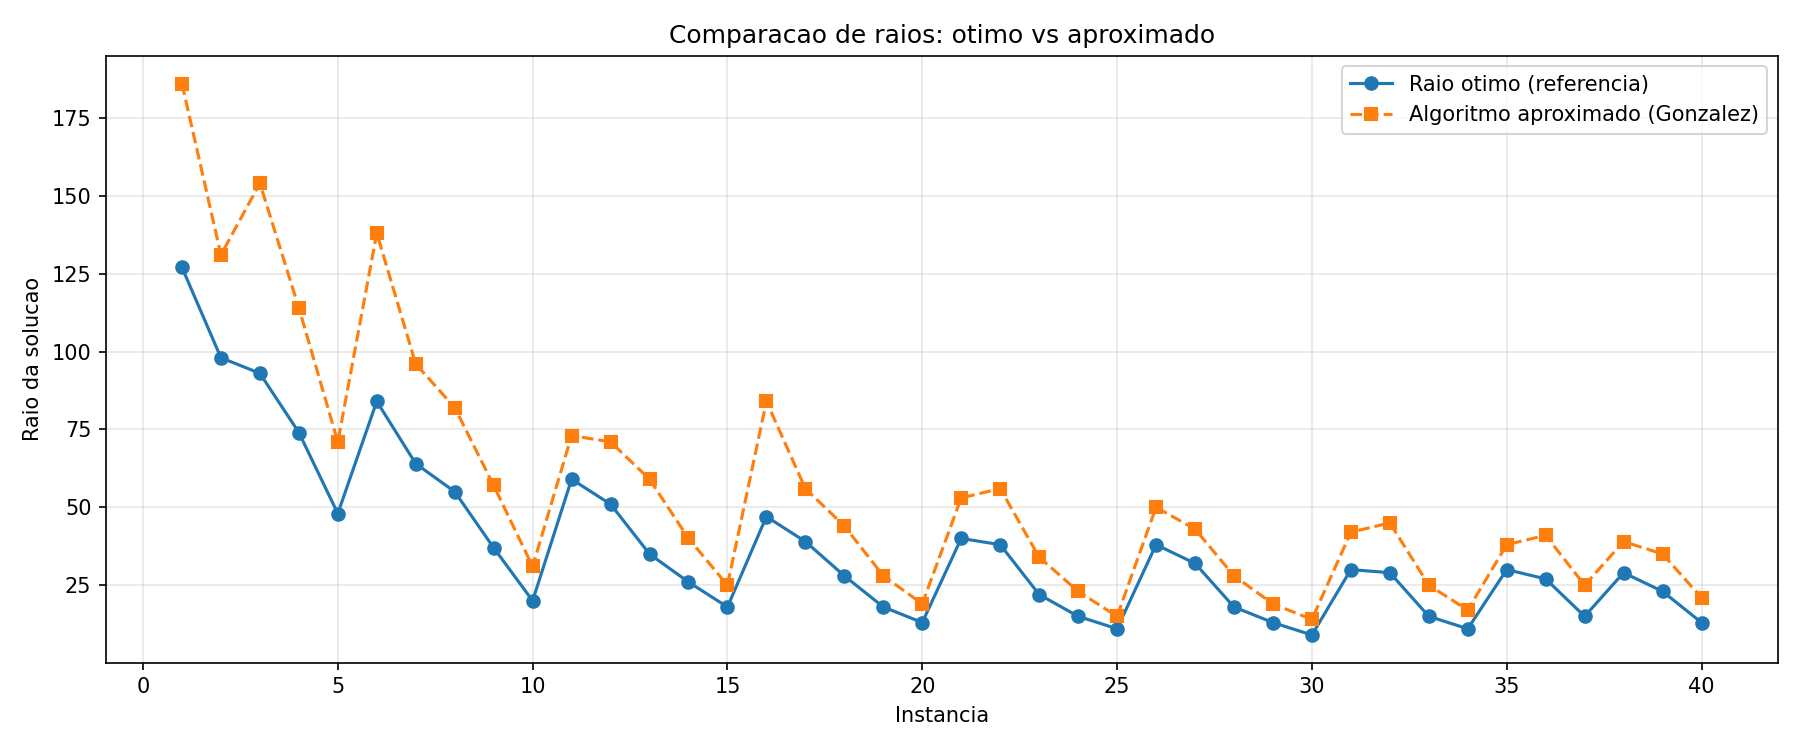
\includegraphics[width=0.95\textwidth]{figuras/raios_comparacao.png}
  \caption{Comparação entre o raio ótimo de referência e o raio obtido pelo algoritmo aproximado.}
  \label{fig:raios}
\end{figure}

\begin{figure}[H]
  \centering
  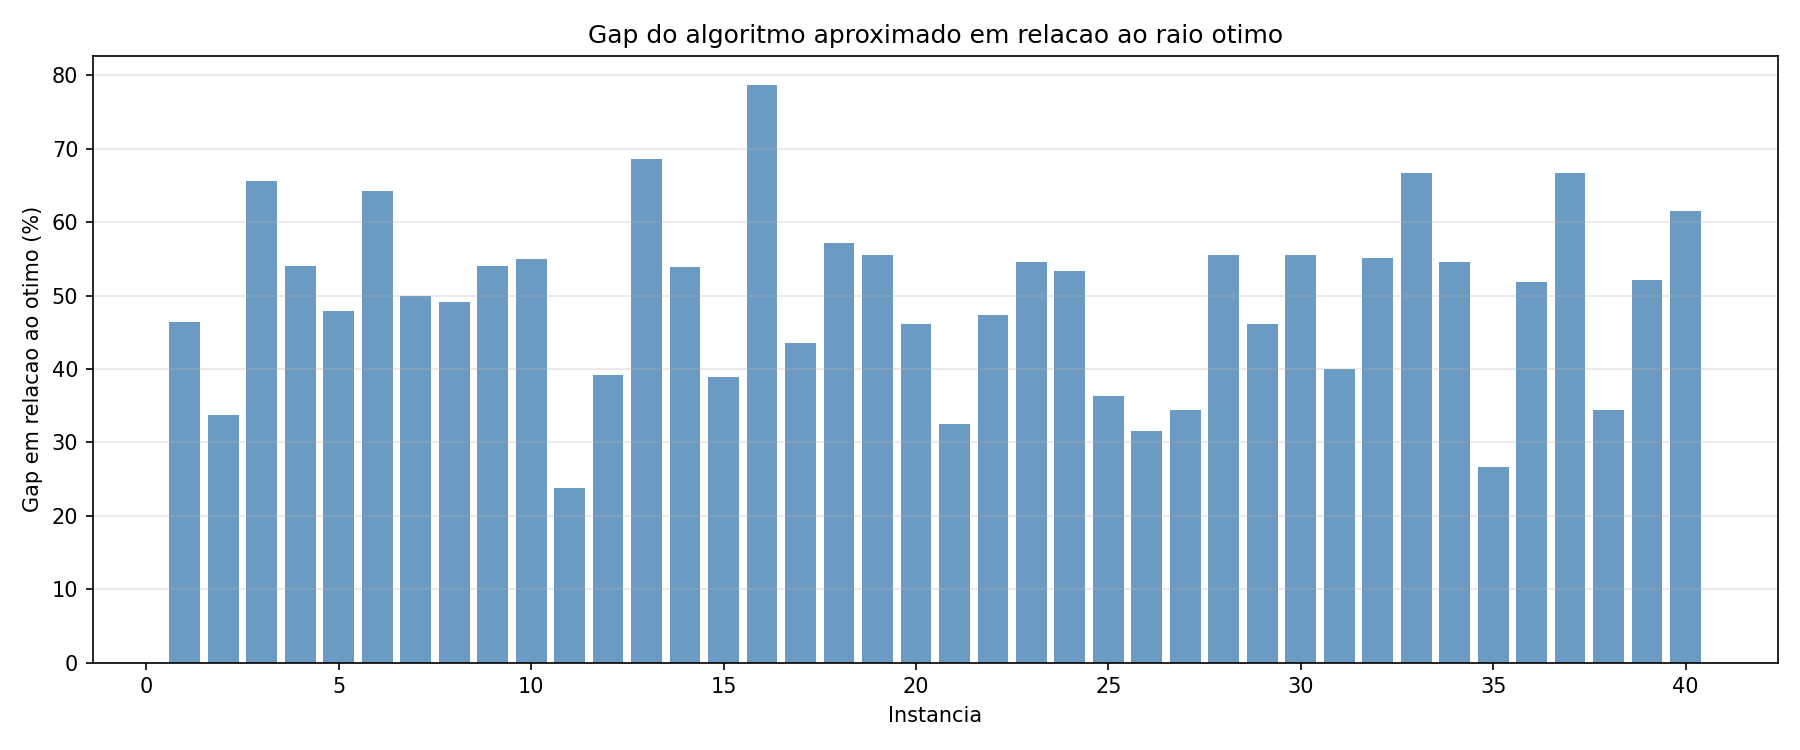
\includegraphics[width=0.95\textwidth]{figuras/gap_aproximado.png}
  \caption{Gap percentual do algoritmo aproximado em relação ao raio ótimo.}
  \label{fig:gap}
\end{figure}

\subsection{Resultados: Tempo de Execução}

A Figura~\ref{fig:tempos} ilustra o comportamento assintótico dos tempos. O algoritmo aproximado permanece abaixo de 2 segundos mesmo para $|V|=900$, enquanto o algoritmo exato cresce de cerca de 0,5~s (instâncias com 100 vértices) para quase 20~s (instância 38, $|V|=900$, $k=5$).

\begin{figure}[H]
  \centering
  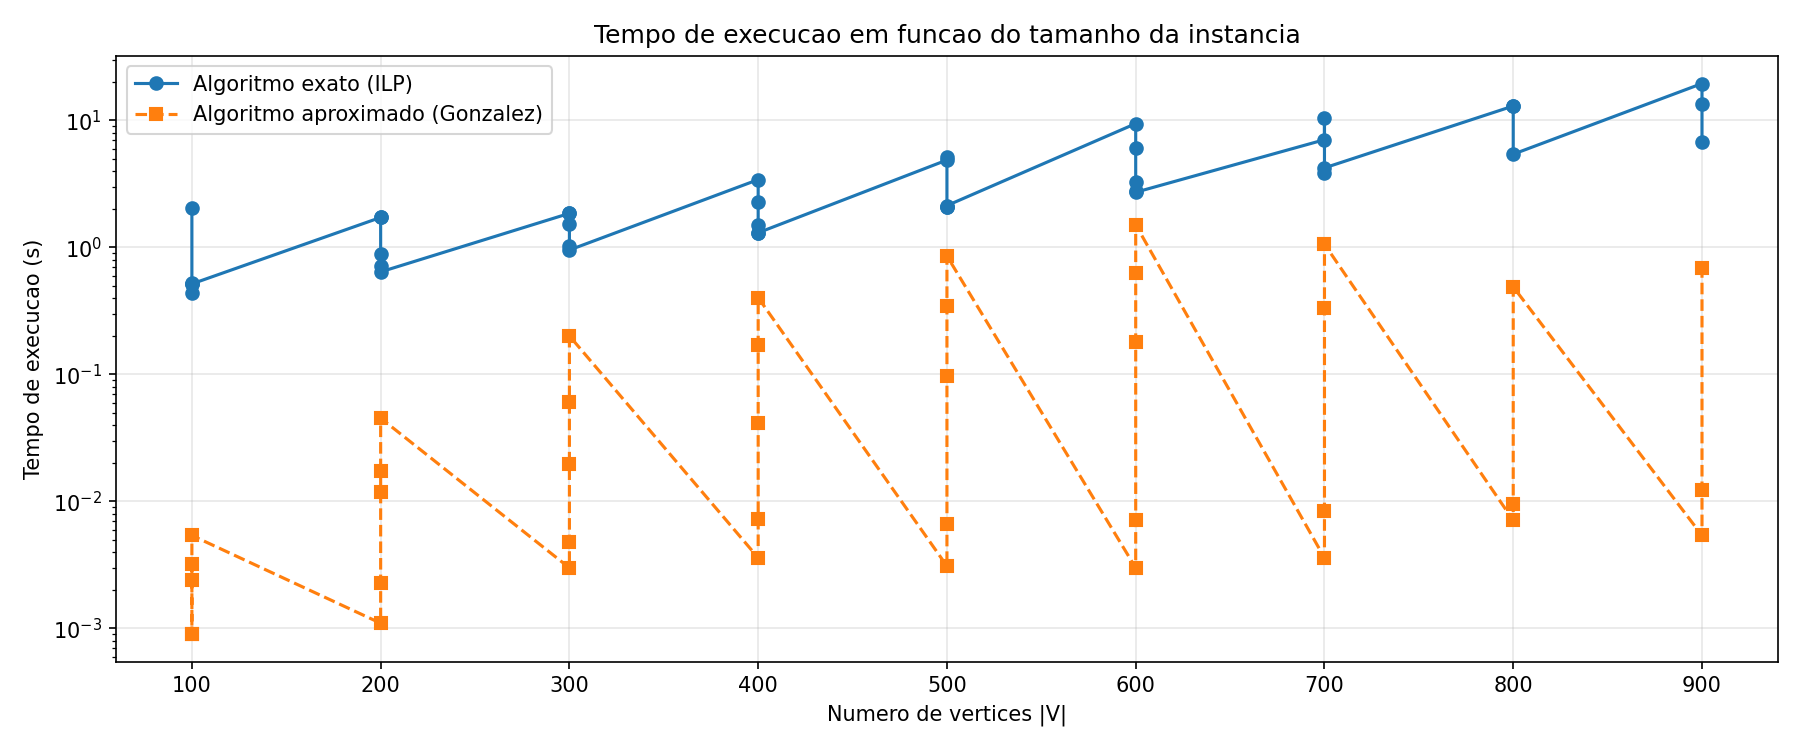
\includegraphics[width=0.95\textwidth]{figuras/tempos_execucao.png}
  \caption{Tempo de execução em função do número de vértices (escala logarítmica).}
  \label{fig:tempos}
\end{figure}

Destacam-se os seguintes pontos:
\begin{itemize}
  \item Para $|V| \leq 200$, o exato resolve em menos de 2 segundos na maioria dos casos.
  \item Instâncias com $k$ pequeno e $|V|$ grande (como 26, 31, 35, 38) exigem mais tempo do exato, pois cada chamada ao solver manipula matrizes maiores.
  \item O aproximado escala de forma muito mais favorável, tornando-se a única opção prática para aplicações em tempo real com instâncias extensas.
\end{itemize}

\section{Análise Comparativa}

\subsection{Eficácia}

O método exato é claramente superior em qualidade: reproduz o raio ótimo em 97,5\% das instâncias. O método aproximado sacrifica qualidade em favor da velocidade, produzindo soluções entre 1,24 e 1,79 vezes piores que o ótimo na maioria dos casos.

Em aplicações onde o custo de um raio adicional é alto (por exemplo, tempo máximo de transporte de pacientes), o algoritmo exato é preferível sempre que o tempo de resposta for aceitável.

\subsection{Eficiência}

O algoritmo de Gonzalez é de 2 a 4 ordens de magnitude mais rápido que o exato nas instâncias maiores. Para $|V|=900$, o exato demanda até 19,5~s enquanto o aproximado resolve em menos de 0,01~s quando $k$ é pequeno.

A relação custo-benefício favorece o aproximado quando:
\begin{itemize}
  \item O tamanho da instância excede algumas centenas de vértices e o tempo de resposta é crítico.
  \item Uma solução razoável é suficiente e o fator 2 de aproximação é aceitável.
  \item É necessário resolver repetidamente o problema com parâmetros variáveis.
\end{itemize}

\subsection{Comportamento com o Crescimento de $|V|$}

Conforme $|V|$ aumenta, o tempo do exato cresce de forma superlinear, refletindo o aumento do número de variáveis e restrições no modelo de programação inteira. O tempo do aproximado cresce quadraticamente com $n$, mas com constante muito menor.

Para instâncias com $k$ proporcional a $n$ (como a instância 30 com $k=200$ e $|V|=600$), o aproximado também aumenta seu tempo (até 1,5~s), ainda assim permanecendo abaixo do exato.

\section{Estrutura do Projeto}

\begin{lstlisting}
tgc-cc-tp02-k-centers/
  pom.xml
  data/                  # Instancias pmed1..pmed40
  src/main/java/br/puc/tgc/kcentros/
    Main.java                # Ponto de entrada
    CarregadorInstancias.java # Leitura e Floyd-Warshall
    KCentrosExato.java       # Algoritmo exato (PLI com ojAlgo + busca binaria)
    KCentrosAproximado.java  # Algoritmo de Gonzalez
    BaixadorDados.java       # Download das instancias
    Experimentos.java        # Execucao dos experimentos
    GeradorGraficos.java     # Geracao de graficos
  results/
    resultados.csv       # Resultados tabulados
  relatorio/
    relatorio.tex        # Este relatorio
    figuras/             # Graficos em PNG
\end{lstlisting}

\section{Conclusão}

Este trabalho implementou e comparou duas abordagens para o problema dos $k$-centros. O algoritmo exato, baseado em busca binária e programação linear inteira com ojAlgo, demonstrou alta eficácia ao encontrar o raio ótimo em praticamente todas as instâncias testadas, com tempo de execução crescente conforme o tamanho da instância. O algoritmo aproximado de Gonzalez mostrou-se extremamente eficiente, porém com perda significativa de qualidade nas soluções.

A escolha entre os métodos depende do contexto da aplicação: quando a otimalidade é essencial e o tempo é secundário, o método exato é indicado; quando a velocidade é prioritária e soluções subótimas são toleráveis, o método aproximado é mais adequado.

\begin{thebibliography}{9}
\bibitem{gonzalez1985}
T.~F. Gonzalez.
Clustering to minimize the maximum intercluster distance.
\textit{Theoretical Computer Science}, 38:293--306, 1985.

\bibitem{orlib}
J.~E. Beasley.
OR-Library: p-median test problems.
\url{http://people.brunel.ac.uk/~mastjjb/jeb/orlib/pmedinfo.html}.
\end{thebibliography}

\newpage
\appendix
\section{Tabela Completa de Resultados}
\label{sec:apendice}

\begin{table}[H]
\centering
\caption{Resultados experimentais para as 40 instâncias.}
\label{tab:resultados}
\small
\begin{tabular}{rrrrrrr}
\toprule
Inst. & $|V|$ & $k$ & Ótimo & Exato & Aprox. & Gap (\%) \\
\midrule
01 & 100 & 5   & 127 & 127 & 186 & 46,46 \\
02 & 100 & 10  & 98  & 98  & 131 & 33,67 \\
03 & 100 & 10  & 93  & 93  & 154 & 65,59 \\
04 & 100 & 20  & 74  & 74  & 114 & 54,05 \\
05 & 100 & 33  & 48  & 48  & 71  & 47,92 \\
06 & 200 & 5   & 84  & 84  & 138 & 64,29 \\
07 & 200 & 10  & 64  & 64  & 96  & 50,00 \\
08 & 200 & 20  & 55  & 55  & 82  & 49,09 \\
09 & 200 & 40  & 37  & 37  & 57  & 54,05 \\
10 & 200 & 67  & 20  & 20  & 31  & 55,00 \\
11 & 300 & 5   & 59  & 59  & 73  & 23,73 \\
12 & 300 & 10  & 51  & 51  & 71  & 39,22 \\
13 & 300 & 30  & 35  & 36  & 59  & 68,57 \\
14 & 300 & 60  & 26  & 26  & 40  & 53,85 \\
15 & 300 & 100 & 18  & 18  & 25  & 38,89 \\
16 & 400 & 5   & 47  & 47  & 84  & 78,72 \\
17 & 400 & 10  & 39  & 39  & 56  & 43,59 \\
18 & 400 & 40  & 28  & 28  & 44  & 57,14 \\
19 & 400 & 80  & 18  & 18  & 28  & 55,56 \\
20 & 400 & 133 & 13  & 13  & 19  & 46,15 \\
21 & 500 & 5   & 40  & 40  & 53  & 32,50 \\
22 & 500 & 10  & 38  & 38  & 56  & 47,37 \\
23 & 500 & 50  & 22  & 22  & 34  & 54,55 \\
24 & 500 & 100 & 15  & 15  & 23  & 53,33 \\
25 & 500 & 167 & 11  & 11  & 15  & 36,36 \\
26 & 600 & 5   & 38  & 38  & 50  & 31,58 \\
27 & 600 & 10  & 32  & 32  & 43  & 34,38 \\
28 & 600 & 60  & 18  & 18  & 28  & 55,56 \\
29 & 600 & 120 & 13  & 13  & 19  & 46,15 \\
30 & 600 & 200 & 9   & 9   & 14  & 55,56 \\
31 & 700 & 5   & 30  & 30  & 42  & 40,00 \\
32 & 700 & 10  & 29  & 29  & 45  & 55,17 \\
33 & 700 & 70  & 15  & 15  & 25  & 66,67 \\
34 & 700 & 140 & 11  & 11  & 17  & 54,55 \\
35 & 800 & 5   & 30  & 30  & 38  & 26,67 \\
36 & 800 & 10  & 27  & 27  & 41  & 51,85 \\
37 & 800 & 80  & 15  & 15  & 25  & 66,67 \\
38 & 900 & 5   & 29  & 29  & 39  & 34,48 \\
39 & 900 & 10  & 23  & 23  & 35  & 52,17 \\
40 & 900 & 90  & 13  & 13  & 21  & 61,54 \\
\bottomrule
\end{tabular}
\end{table}

\end{document}
